\documentclass[11pt]{article}
\pdfinfoomitdate=1\pdftrailerid{}
\usepackage[letterpaper,margin=.7in,headheight=15pt,headsep=18pt,footskip=24pt]{geometry}
\usepackage[T1]{fontenc}
\usepackage{lmodern,amsmath,amssymb,array,booktabs,fancyhdr,tikz}
\renewcommand{\familydefault}{\sfdefault}
\setlength{\parindent}{0pt}\setlength{\parskip}{6pt}
\pagestyle{fancy}\fancyhf{}
\fancyhead[L]{\small Week 97 / Square remainders / K--1 adult guide}
\fancyfoot[L]{\scriptsize Bellingham Math Circle / Week 97 / W97-K-FAC-v1}
\fancyfoot[R]{\thepage}
\renewcommand{\headrulewidth}{0pt}
\newcommand{\head}[1]{\par\textbf{\large #1}\par}
\newcommand{\sub}[1]{\par\textbf{#1}\par}
% Generated by check_guide.py from independent enumeration.
\newcommand{\Pone}{1, 0, 1, 0, 1, 0}
\newcommand{\Ptwo}{0:\{2, 4\};\quad 1:\{1, 3, 5\}}
\newcommand{\Pthree}{0, 2, 2, 3}
\newcommand{\Recttotals}{12, 6, 10, 15}
\newcommand{\Pfour}{1, 1, 0, 1, 1, 0}
\newcommand{\Pfive}{1, 4, 3, 4, 1, 0}
\newcommand{\Psix}{0:\{6\};\quad 1:\{1, 5\};\quad 3:\{3\};\quad 4:\{2, 4\}}
\newcommand{\Pseven}{1, 0, 1, 0, 1}
\newcommand{\Peighta}{1}
\newcommand{\Peightb}{0}
\newcommand{\Ringcounts}{8, 16}
\newcommand{\Pten}{1}
\newcommand{\Peleven}{0:\{4\};\quad 1:\{1, 3, 5\};\quad 4:\{2, 6\}}

\begin{document}
\head{Mathematical overview: what a leftover can tell us}
\textbf{Squares restrict the leftovers.} For a filled $n\times n$ square, remove any $m$ tiles at a time until fewer than $m$ remain. Here $n$ is a whole-number side length and $m>0$; the leftover can be zero. The choice of tiles does not affect it. Squares leave only 0 or 1 in groups of 3 or 4, and only 0, 1, 3 or 4 in groups of 6. These restrictions are about squares, not arbitrary piles or rectangles.

\textbf{Why a finite list suffices.} Adding $m$ to a side adds two $n\times m$ strips and an $m\times m$ corner. Each added region splits into whole groups of $m$, so sides $n$ and $n+m$ have the same leftover. Sides 1 through $m$ therefore cover every possibility, including side zero's leftover. The student cards themselves start at 1, not zero. For groups of 4, an even-sided square splits into $2\times2$ blocks. An odd-sided square has an even square inside, two equal even-length arms that pair into groups of 4, and one corner tile: only that corner remains.

\textbf{One result can hide several squares.} A secret is not always recoverable. The correct answer names \emph{all} allowed side cards with that leftover, not just the chosen card. The group size and the allowed cards both matter. For a later route, every odd square leaves 1 in groups of 8: its rings have $8,16,24,\ldots$ tiles, all full groups, leaving the middle tile.

\textbf{Discovery and evidence.} K--1 reaches restricted leftovers, ambiguity, and a first geometric explanation; see the base guide's overview (p.\ 1) for the older tables' prime/composite destination. A child's build is an experiment; ``I think this always happens'' is a conjecture. Checking every allowed card proves a finite game answer. ``These blocks all go away, and this corner stays'' can explain a general pattern with objects; merely testing more squares does not. No modular notation or multiplication facts are required of the children.

\head{Preparation and access}
\textbf{Status.} Unpiloted and physically unrehearsed. Tile fit, cutting, screen concealment, card handling, adult procedures and timings still need a real rehearsal.

\textbf{Per pair.} Use the week's 64 square tiles, ideally 1-inch (25.4\,mm), a whiteboard and pen, and scrap paper. Add one cup and one upright folder screen. Two colors are useful for rings; 32 of each suffice. Reuse tiles between builds. The six printed picture cards replace the base kit's hand-marked input cards at this table; no extra deck is needed.

\textbf{Print.} From the draft \texttt{k-1.pdf}, print pages 1--11 for the tasks, page 12 separately as the workboard, and one copy of page 13 per pair to cut into six side cards (58 by 74\,mm). First-visit minimum: pages 1--3, 12 and 13; keep page 7 available as an easier entry. US Letter, single-sided, Actual Size. The board is $6\times6$, 156\,mm across; board and group-card cells are 26\,mm. Measure one cell and try a tile before use. The little square pictures are records, not tile mats. Keep page 12 loose beside the current problem page; cut only the side-card sheet. Allow 5--10 extra minutes per pair for cutting and fit checks beyond the base week's kit preparation. No separate Week 97 materials PDF is needed.

\newpage
\head{Launch together, then learn the table action}
Join the base guide's whole-group launch (p.\ 2): handle the tiles, see the $3\times3$ square in groups of 4 and the empty square, and make a legal attempt. At the K--1 table bridge the words: ``input'' is the side, ``bundle'' is a group, and ``output'' is the leftover. Page 1 already records the shared example; do not treat its grey 1 as a new puzzle.

\textbf{A non-task demonstration, about 3 minutes.} On the whiteboard draw five tile-sized spaces in a row (at least 26\,mm each). This temporary group-of-5 mat is not a student task. Fill a side-3 square on the loose board, including its middle. Have a child move any five tiles onto the five spaces, then into the cup. Four tiles remain; trying to fill the mat again leaves a space empty. Those four are the leftover, whether on the board or the partly filled mat. Record 4 in a box beneath side 3.

\begin{center}
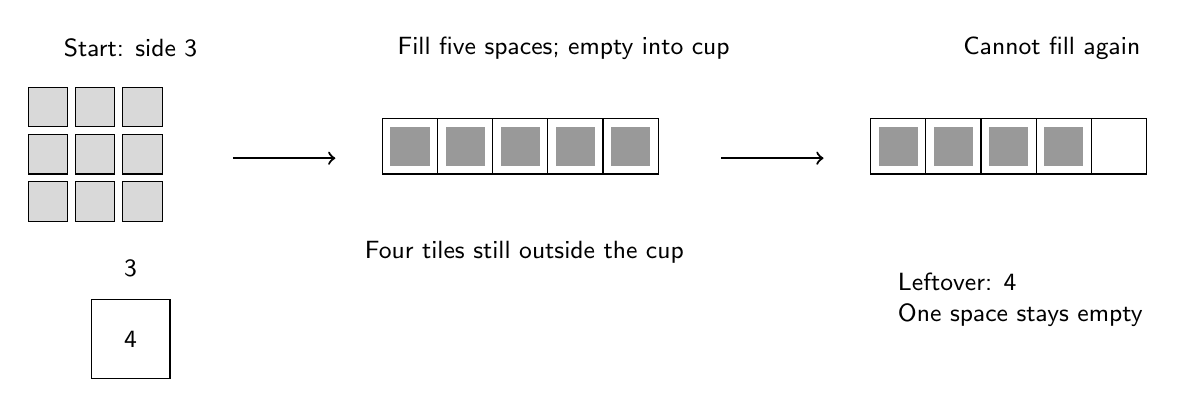
\begin{tikzpicture}[x=1mm,y=1mm,font=\small]
\node at (13,22) {Start: side 3};
\foreach \x in {0,1,2}\foreach \y in {0,1,2}
 {\filldraw[fill=black!15] (\x*6,\y*6) rectangle +(5,5);}
\draw[->,thick] (26,8)--(39,8);
\node at (68,22) {Fill five spaces; empty into cup};
\foreach \x in {0,1,2,3,4}
 {\draw (45+\x*7,6) rectangle +(7,7);\fill[black!40] (46+\x*7,7) rectangle +(5,5);}
\node[align=center] at (63,-4) {Four tiles still outside the cup};
\draw[->,thick] (88,8)--(101,8);
\node at (130,22) {Cannot fill again};
\foreach \x in {0,1,2,3,4} {\draw (107+\x*7,6) rectangle +(7,7);}
\foreach \x in {0,1,2,3} {\fill[black!40] (108+\x*7,7) rectangle +(5,5);}
\node at (13,-6) {3};\draw (8,-20) rectangle +(10,10);\node at (13,-15) {4};
\node[align=left] at (126,-10) {Leftover: 4\\One space stays empty};
\end{tikzpicture}
\end{center}
Use the printed group card for each real task. Full groups go in the cup; partial groups never do. Tiles may come from anywhere: the card's rectangular shape does not restrict their positions in the square. Reset with all the square's tiles before changing the group size. Let the children choose which square to try and which tiles to move.

\textbf{Prerequisites and staffing.} One adult anchored to the K--1 table, supporting up to two pairs, reads every task aloud and writes a child's result when asked. Children count along sides up to 6 and recognize or count groups up to 8; Problem 8 adds side labels 9 and 10. They need not count 25 or 36 tiles or multiply. The adult can point to the matching record box, but children build, choose secrets, test candidates and decide what to circle. If the adult is choosing every move, stay with a smaller concrete collection. With three children, rotate maker, guesser and checker.

\textbf{A first hour, not a race.} Allow 5 minutes for movement, 5 for the shared launch, 3 for the table demonstration, about 15 for Problem 1, 15 for Problem 2, 10 for contrasting rectangles in Problem 3, and 7 for sharing and reset. Pool the square cases between pairs if handling is slow; an unfinished collection can resume next time. Preserve time for the game rather than requiring every square first. Problem 7 is an alternative entry, not an additional obligation. Return to Problems 4--6 on another visit. Offer Problem 8 when children want a reason beyond examples; Problems 9--11 form a later ring-and-secret investigation. Finishing every page is not the goal.

\textbf{Before a secret round.} Lay out only the allowed cards; remove card 6 for Problem 2. Choose behind the screen; keep the whole deck, square, spare tiles and cup hidden so neither the missing card nor the number of groups gives a clue. Bring only the leftover forward, rearranged into a loose pile. Put its number in the left box of one row; circle every possible side in that row. Reveal the chosen card, check disputed candidates by rebuilding, then swap roles. The four rows are four rounds, not four different required leftovers.

\newpage
\head{Problems 1--6: collections and secret squares}
All lists follow the pictures from left to right. Side numbers describe the edge, not the tile total.

\sub{Problem 1, page 1: groups of 4}
For sides 1--6 the leftovers are $\Pone$. Circle 0 and 1 only. The prefilled side-3 answer is correct. The overview's blocks-and-corner argument rules out 2 and 3 for \emph{every} square; testing the six pictured cases alone does not.

\textit{Hints, only if needed:} ``Is your square filled in, or only outlined?'' ``Could any full group still go into the cup?'' Accept a demonstration instead of a spoken rule.

\sub{Problem 2, page 2: all possible cards, not a lucky guess}
With cards 1--5 and groups of 4: $\Ptwo$. Leftovers 2 and 3 cannot occur. These collections contain every allowed card. Children can read Problem 1 backward: ``These three squares all left one.'' The revealed card belongs in the answer but need not be the only answer.

\textit{Hints:} ``Could a different allowed card leave the same pile?'' ``Which cards have you checked?'' Later, allow card 6: it joins the leftover-0 collection; the leftover-1 collection stays unchanged.

\sub{Problem 3, page 3: what rectangles can do}
The printed rectangles are $4\times3$, $3\times2$, $5\times2$, $5\times3$ (width by height). Their leftovers in groups of 4 are $\Pthree$. Thus rectangles can leave 2 and can leave 3. The tile totals are $\Recttotals$; children need not calculate them. The two middle builds witness 2, and the last witnesses 3. One successful build proves each ``can'' claim.

\textit{Hints:} ``Which of these has a different number of tiles along the two edges?'' ``Can you show a rectangle whose last group will not fill?'' Later, invent another rectangle with the same leftover.

\sub{Problem 4, page 4: groups of 3}
For sides 1--6: $\Pfour$; circle 0 and 1. The first three sides cover a complete repeat. For an object explanation, remove strips three tiles wide; each strip breaks into rows of three. Continue until the remaining corner is a square of side 0, 1 or 2. Its 0, 1 or 4 tiles leave 0, 1 or 1. So no square can leave 2.

\textit{Hints:} ``Can you fill the card using tiles from different rows?'' ``What happens to a whole strip three tiles wide?'' The straight group card is a counting aid, not a rigid piece to fit inside the square. Side 6 takes 12 card-fills: share that case or save it rather than let repeated handling displace comparison.

\sub{Problem 5, page 5: groups of 6}
For sides 1--6: $\Pfive$; circle 0, 1, 3 and 4. Sides 1--6 are a whole repeat, so 2 and 5 are impossible for any square. Children can explain the finite claim by pointing to one checked result for every side; the strip argument in the overview extends it to all sides.

\textit{Hints:} ``Where could an unchecked side fit in your collection?'' ``Is 4 still a leftover when the card needs 6?'' An unfinished card belongs outside the cup.

\sub{Problem 6, page 6: the secret game changes}
With cards 1--6 and groups of 6: $\Psix$. Leftovers 2 and 5 have no possible card. All six cards are accounted for, so these are complete answers. One and four hide two cards each; zero and three identify the card exactly.

\textit{Hints:} ``Which entries in Problem 5 match this leftover?'' ``Did changing the group size change what you could know?'' Compare with Problem 2 without changing the allowed cards mid-round.

\newpage
\head{Problems 7--11: reasons, rings and a return to the game}
\sub{Problem 7, page 7: groups of 2}
For sides 1--5: $\Pseven$. Sides 1, 3 and 5 leave 1. With an even side, pair adjacent tiles within each row. With an odd side, pairing within rows leaves one tile per row, an odd column; pair those until one remains. This explains the result for any square, not just the five pictured ones.

\textit{Hints:} ``Can every tile find a partner?'' ``What shape is left when each row has made its pairs?'' Begin with smaller squares if handling is slow. Compare with Problem 1: squares have the same leftovers in groups of 2 and 4, unlike arbitrary piles.

\sub{Problem 8, page 8: beyond the kit}
The side-9 square leaves $\Peighta$ in groups of 4; side 10 leaves $\Peightb$. Adult check: $81=20\cdot4+1$ and $100=25\cdot4$. Neither square fits one 64-tile kit; follow ``without building'' and reason on the pictures.

The $10\times10$ drawing splits into $2\times2$ blocks. In the $9\times9$ drawing, mark an $8\times8$ corner square, two arms of eight tiles, and the last corner: $81=64+8+8+1$. The inner square and arms make whole groups of 4; only the corner remains. Children may draw block outlines or point as the adult records their explanation.

\textit{Hints:} ``Where could you see groups of four without counting every tile?'' ``What remains around an even-sided square?'' An earlier pattern predicts the answers; the blocks and arms explain them.

\sub{Problem 9, page 9: build from the middle}
Sides 1, 3 and 5 all leave 1 in groups of 8. The new rings contain $\Ringcounts$ tiles. The first ring fills the group card once; the next fills it twice. The middle tile remains. Build on the table, not inside the corner-anchored board. Use two colors for successive rings; with one color, remove one ring at a time, rebuilding before the next whole-square trial.

\textit{Hints:} ``Which tile was there before any ring?'' ``Can the new ring leave anything behind?'' Have children show full rings going into the cup before naming a pattern. Build one square at a time.

\sub{Problem 10, page 10: the next ring}
The $7\times7$ square leaves $\Pten$ in groups of 8. Its outer ring adds 24 tiles, three complete groups, to the previous square. Altogether $49=1+8+16+24=6\cdot8+1$. Children can point to the middle and the three colored rings. An optional 49-tile check fits the kit, but use the table: the board stops at side 6. Borrow page 9's group-of-8 card.

\textit{Hints:} ``What was added around the square you already know?'' ``Can you divide that ring into full groups?'' For a ready child, the $k$th ring has $8k$ tiles: its top and bottom rows have $2k+1$ each, and the two remaining sides have $2k-1$ each. Their sum is $8k$. Thus every odd square, however large, leaves its single center tile.

\sub{Problem 11, page 11: rings meet hidden cards}
With cards 1--6 and groups of 8: $\Peleven$. Leftovers 2, 3, 5, 6 and 7 have no allowed card. The six tested cards exhaust the choices. The rings explain why all three odd cards share leftover 1; the even cards must also be tested. Sides 2, 4 and 6 leave 4, 0 and 4.

\textit{Hints:} ``Which cards can you settle with rings?'' ``What about the cards without a single middle tile?'' Optional return: add a hand-marked side-7 card. It joins the leftover-1 group, now four possibilities; a drawing suffices. This connects to the older table.

\textbf{Where it goes.} After the pages are approved, this section replaces ``K--1 route (adult-led, no packet, about 15 minutes)'' on page 2 of \texttt{week-97-facilitator.pdf} (W97-FAC-v3); keep that guide's whole-group launch and older-band overview.
\end{document}
